\documentclass{tufte-handout}
\usepackage{booksprint}

\title[Short Title]{Sprint Beyond the Book - Template}
\author{John Hammersley and Mary Anne Baynes}
\date{\today}

\begin{document}
\maketitle
\logos

\section{Introduction}

This is the writing template for the ``Sprint Beyond the Book'' sessions at SSP 2016. We invite you to join our team of science fiction authors, scholars, digital publishers, journalists, and technologists to write, edit, assemble and publish a book about the future of scholarly publishing on-the-fly in 72 hours. 

We will employ a variety of collaborative technologies and explore the idea of writing as a performance. In order to pull off this ambitious plan, we need your help! Please stop by to help brainstorm, write, or edit contributions. 

Each concurrent session will confront participants with different provocation about the future of scholarly publishing.

\section{Getting Started with Overleaf}

Welcome to Overleaf! Simply write your text on the left and see it composed automatically in the preview window on the right. Some examples of commonly used commands and features are listed below, to help you get started.

If you have a question, please use the help menu (``?'') on the top bar to search for help or to ask us a question.

\subsection{How to create Sections and Subsections}

Use section and subsections to organize your document. Simply use the section and subsection buttons in the toolbar to create them, and we'll handle all the formatting and numbering automatically.

\subsection{How to add Lists}

You can make lists with automatic numbering:
\begin{enumerate}
\item Like this,
\item and like this.
\end{enumerate}
or with bullet points:
\begin{itemize}
\item Like this,
\item and like this.
\end{itemize}
using the buttons in the toolbar.

\subsection{Special characters}

Some common characters have special meanings in \LaTeX{}:

\begin{itemize}
\item \% percent sign
\item \# hash sign
\item \& ampersand
\item \$ dollar sign
\end{itemize}

If you just type these you'll get an error; you'll need to precede these symbols with a backslash in order for it to appear in the output (as in the examples above).

You can include accented characters (e.g. if you were writing your résumé) in the usual way.

\subsection{Adding web links (URLs)}

As URLs can sometimes contain special characters that can cause compilation errors, it's best to include web links as follows:

\url{https://www.overleaf.com}

\subsection{How to add Comments}

Comments which appear in the editor pane (but not in the final pdf) can be added to your project by clicking on the comment icon in the toolbar above. These are useful for adding notes to the editors (or for editors to leave notes for the author).% * <john.hammersley@gmail.com> 2016-06-01T09:54:16.211Z:
%
% Here's an example comment!
%
To reply to a comment, simply click the reply button in the lower right corner of the comment, and you can close them when you're done.

\subsection{How to include Figures}

First you have to upload the image file from your computer using the `Add Files' option in the project menu. Then use the includegraphics command to include it in your document. Use the figure environment and the caption command to add a number and a caption to your figure. See the code for Figure \ref{fig:frog} in this section for an example.

\begin{figure}
\centering
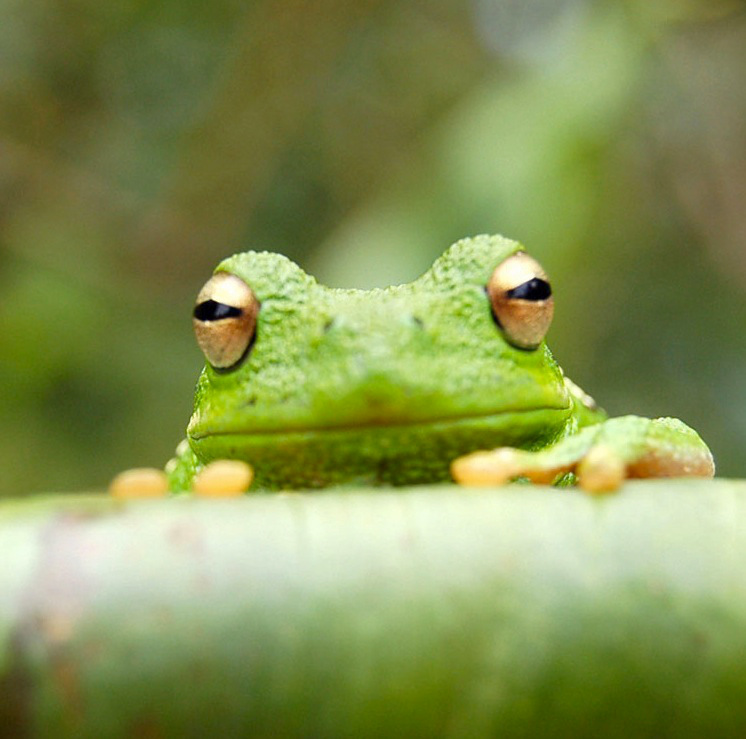
\includegraphics[width=0.8\textwidth]{frog.jpg}
\caption{\label{fig:frog}This frog was uploaded via the project menu.}
\end{figure}

\subsection{How to include citations to  references}

Here is an example of a citation\cite{tufte1983visual} -- the reference appears in the margin. The actual entry itself is stored in the \texttt{references.bib} file. 

Rather than agonizing over how to write each entry, you can look up a reference in Google Scholar, then click on the `Cite' link below the item you need. In the pop-up window that appears, you should see a `BibTeX' link. Click on that, and you can copy and paste the code into your \texttt{references.bib file}. Here's a video to help you along: \url{https://www.overleaf.com/help/97}

\subsection{How to include notes and figures in the margin}

\marginnote{Here is an example of a note in the margin.}

\lipsum[1] % Dummy text - delete this line to remove.

\begin{marginfigure}
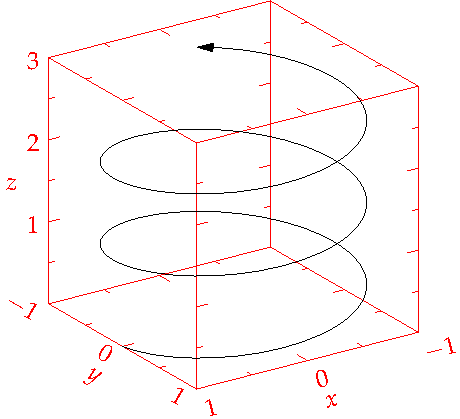
\includegraphics{helix}
\caption{Here we've included a margin figure example with caption!}
\end{marginfigure}

\lipsum[2] % Dummy text - delete this line to remove.

% The bibliography style.
\bibliographystyle{apalike}

% If you DO want the full list of references to be printed at the end.
% \bibliography{references}

% If you do NOT want the full list of references to be printed at the end.
\nobibliography{references}

\end{document}